\begin{figure}[htbp]
\centering
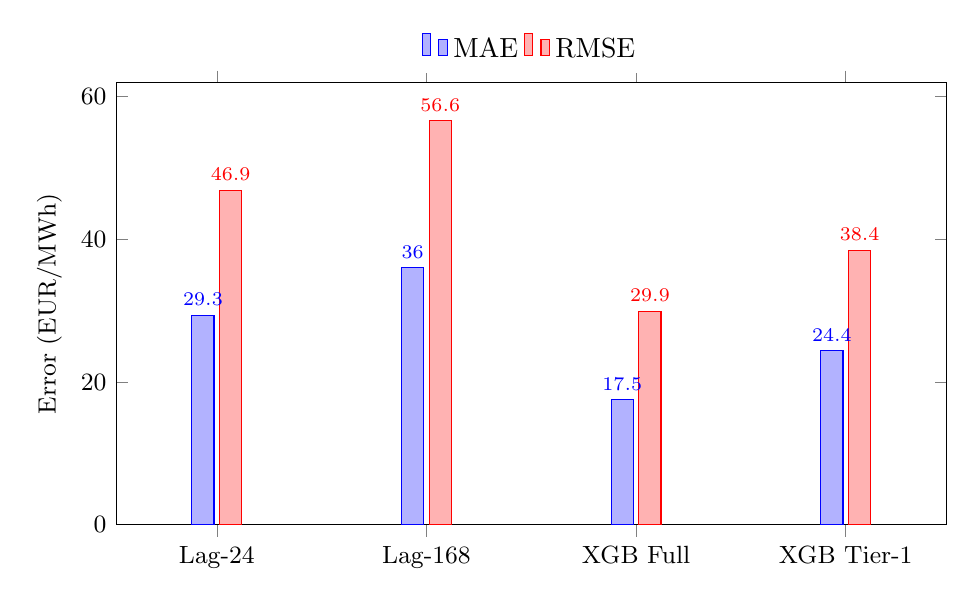
\begin{tikzpicture}
\begin{axis}[
  ybar,
  bar width=8pt,
  width=\textwidth,
  height=7.2cm,
  ylabel={Error (EUR/MWh)},
  symbolic x coords={Lag-24,Lag-168,XGB Full,XGB Tier-1},
  xtick=data,
  ymin=0,
  ymax=62,
  enlarge x limits=0.16,
  legend style={at={(0.5,1.02)},anchor=south,legend columns=2,draw=none},
  nodes near coords,
  nodes near coords style={font=\scriptsize,/pgf/number format/fixed,/pgf/number format/precision=1},
  tick label style={font=\small},
  label style={font=\small}
]
\addplot coordinates {(Lag-24,29.3291) (Lag-168,36.0141) (XGB Full,17.5122) (XGB Tier-1,24.3606)};
\addplot coordinates {(Lag-24,46.8553) (Lag-168,56.5983) (XGB Full,29.8691) (XGB Tier-1,38.4137)};
\legend{MAE,RMSE}
\end{axis}
\end{tikzpicture}
\caption{Point-forecast accuracy in the frozen 2026 holdout (\(N=5{,}087\) common hourly observations). Full XGBoost has the lowest MAE and RMSE, while Tier-1 XGBoost remains more accurate than both naive benchmarks.}
\label{fig:holdout_accuracy}
\end{figure}
